\documentclass[12pt,a4paper]{report}

\usepackage[utf8]{inputenc}
\usepackage[T1]{fontenc}
\usepackage{babel}
\usepackage{geometry}
\usepackage[protrusion=true,expansion=false]{microtype}
\usepackage{graphicx}
\usepackage[table]{xcolor}
\usepackage{booktabs}
\usepackage{array}
\usepackage{tabularx}
\usepackage{multirow}
\usepackage{enumitem}
\usepackage{setspace}
\usepackage{fancyhdr}
\usepackage{titlesec}
\usepackage{tocloft}
\usepackage{hyperref}
\usepackage{float}
\usepackage{mdframed}
\usepackage{parskip}
\usepackage{ragged2e}
\usepackage{longtable}
\usepackage{tikz}

\raggedbottom
\graphicspath{{images/}}
\setlength{\headheight}{15pt}
\geometry{top=2.5cm, bottom=2.5cm, left=2.5cm, right=2.5cm}

\definecolor{mainblue}{RGB}{31,111,120}
\definecolor{accentbrown}{RGB}{138,90,34}
\definecolor{lightgray}{RGB}{245,245,245}
\definecolor{darkgray}{RGB}{80,80,80}
\definecolor{ucblue}{RGB}{31,95,165}
\definecolor{ucpurple}{RGB}{83,74,183}
\definecolor{ucgreen}{RGB}{15,110,86}
\definecolor{ucamber}{RGB}{186,117,23}
\definecolor{uccoral}{RGB}{153,60,29}

\pagestyle{fancy}
\fancyhf{}
\fancyhead[L]{\small\textcolor{mainblue}{LudoHeritage}}
\fancyhead[R]{\small\textcolor{darkgray}{\leftmark}}
\fancyfoot[C]{\thepage}
\fancyfoot[L]{\small LudoHeritage -- Projet de Fin d'Année}
\fancyfoot[R]{\small 2024--2025}
\renewcommand{\headrulewidth}{0.4pt}
\renewcommand{\footrulewidth}{0.4pt}

\titleformat{\chapter}[block]
  {\normalfont\huge\bfseries\color{mainblue}}
  {\thechapter.}{1em}{}
  [\vspace{0.5ex}\titlerule]

\titleformat{\section}
  {\normalfont\Large\bfseries\color{mainblue}}
  {\thesection}{1em}{}

\titleformat{\subsection}
  {\normalfont\large\bfseries\color{accentbrown}}
  {\thesubsection}{1em}{}

% UC table command
\newcommand{\uctable}[7]{%
\renewcommand{\arraystretch}{1.55}
\begin{tabular}{|>{\bfseries\color{darkgray}}p{3.8cm}|p{10cm}|}
\hline
\multicolumn{2}{|l|}{\cellcolor{#1!18}\textbf{\textcolor{#1}{#2}}} \\
\hline
Acteur principal   & #3 \\
\hline
Préconditions      & #4 \\
\hline
Postconditions     & #5 \\
\hline
Déroulement        & #6 \\
\hline
Cas d'erreur       & #7 \\
\hline
\end{tabular}
\renewcommand{\arraystretch}{1}}

\begin{document}

%=============================================================================
%  PAGE DE GARDE
%=============================================================================
\begin{titlepage}
\thispagestyle{empty}
\centering
\vspace*{1cm}
{\Large\scshape École Nationale Supérieure d'Informatique\\
et d'Analyse des Systèmes -- RABAT}
\vspace{1.2cm}

{\Huge\bfseries\color{mainblue} LudoHeritage}
\vspace{0.4cm}

{\large\bfseries Plateforme Web Interactive pour la Préservation\\
et l'Exploration du Patrimoine Ludique Mondial}
\vspace{1cm}

\begin{mdframed}[linecolor=mainblue, linewidth=1.5pt,
                 innertopmargin=14pt, innerbottommargin=14pt,
                 innerleftmargin=16pt, innerrightmargin=16pt]
\centering
{\large\bfseries\color{mainblue} LudoHeritage}\\[0.2cm]
{\small\color{darkgray} Encyclopédie Interactive des Jeux Traditionnels}
\end{mdframed}

\vspace{1cm}
\begin{minipage}[t]{0.45\textwidth}
\raggedright
\textit{Soutenu par :}\\[0.3cm]
Prénom \textsc{Nom}
\end{minipage}
\hfill
\begin{minipage}[t]{0.45\textwidth}
\raggedleft
\textit{Membres du jury :}\\[0.3cm]
Hicham \textsc{Salaheddine}\\
Adil \textsc{Bentalb}
\end{minipage}
\vfill
{\large Année universitaire 2024--2025}
\end{titlepage}

%=============================================================================
%  DEDICACE
%=============================================================================
\newpage
\thispagestyle{empty}

% Top rule
\noindent\textcolor{mainblue}{\rule{\linewidth}{1.2pt}}

\vspace*{2.5cm}

\begin{center}
  {\large\bfseries\color{mainblue}\scshape Dédicaces}
\end{center}

\vspace{0.6cm}
\noindent\textcolor{mainblue!40}{\rule{\linewidth}{0.4pt}}
\vspace{1.4cm}

\begin{flushright}
\begin{minipage}{0.72\textwidth}
\setstretch{1.8}
\itshape\large\color{darkgray}

À ma famille, dont le soutien indéfectible\\
a été notre plus grande force.\\[1em]
À mes amis, compagnons de route\\
dans les moments de doute comme de réussite.\\[1em]
À mes enseignants et encadrants,\\
qui ont façonné notre rigueur et notre curiosité.

\end{minipage}
\end{flushright}

\vfill

\noindent\textcolor{mainblue!40}{\rule{\linewidth}{0.4pt}}

\vspace{0.6cm}

\begin{center}
  \textcolor{mainblue}{\large\bfseries\scshape Merci}
\end{center}

\vspace{0.4cm}
\noindent\textcolor{mainblue}{\rule{\linewidth}{1.2pt}}

%=============================================================================
%  REMERCIEMENTS
%=============================================================================
\newpage
\chapter*{Remerciements}
\addcontentsline{toc}{chapter}{Remerciements}
\thispagestyle{fancy}

Nous tenons à exprimer notre sincère gratitude à toutes les personnes qui nous ont
soutenus tout au long de ce projet.

Nous sommes reconnaissants envers notre professeur encadrant \textbf{M.~Hicham SALAHEDDINE},
pour sa confiance, sa disponibilité et les précieux conseils qu'il nous a prodigués.

Nos remerciements vont également à \textbf{M.~Adil BENTALB}, professeur de culture
entrepreneuriale, dont l'enseignement nous a fourni les outils et la rigueur nécessaires
pour mener ce projet avec sérieux et esprit d'initiative.

Enfin, nous exprimons notre reconnaissance envers l'ensemble du corps enseignant et
administratif de l'\textbf{ENSIAS} pour l'environnement d'apprentissage de qualité qu'ils
nous offrent.

%=============================================================================
%  RESUME
%=============================================================================
\newpage
\chapter*{Résumé}
\addcontentsline{toc}{chapter}{Résumé}
\thispagestyle{fancy}

Ce document présente le travail accompli dans le cadre de notre Projet de Fin d'Année.
L'objectif principal était de concevoir et développer une plateforme web dédiée à la
\textbf{sauvegarde et à la découverte des jeux de société traditionnels du monde entier}.

Notre démarche a débuté par une étude fonctionnelle approfondie permettant d'identifier
la problématique et les caractéristiques essentielles du système. Nous avons ensuite
conduit une étude conceptuelle à travers des diagrammes de cas d'utilisation et un
modèle UML, ce qui a facilité la phase d'implémentation. L'application repose sur
\textbf{Spring Boot} côté serveur, \textbf{React} pour l'interface et \textbf{MongoDB}
pour la base de données.

\medskip
\noindent\textbf{Mots-clés :} jeux traditionnels, patrimoine culturel, application web,
intelligence artificielle, Spring Boot, React, MongoDB.



%=============================================================================
%  LISTE DES ABREVIATIONS
%=============================================================================
\newpage
\chapter*{Liste des Abréviations}
\addcontentsline{toc}{chapter}{Liste des Abréviations}
\thispagestyle{fancy}

\renewcommand{\arraystretch}{1.7}
\begin{tabular}{>{\bfseries}p{3.5cm} p{10cm}}
\toprule
\textbf{Abréviation} & \textbf{Désignation} \\
\midrule
API     & Application Programming Interface \\
REST    & Representational State Transfer \\
LLM     & Large Language Model \\
IA      & Intelligence Artificielle \\
UI / UX & User Interface / User Experience \\
JSON    & JavaScript Object Notation \\
HTTP    & HyperText Transfer Protocol \\
CORS    & Cross-Origin Resource Sharing \\
MVC     & Model-View-Controller \\
PFA     & Projet de Fin d'Année \\
DLP     & Digital Ludeme Project \\
SPA     & Single Page Application \\
JWT     & JSON Web Token \\
SGBD    & Système de Gestion de Base de Données \\
\bottomrule
\end{tabular}
\renewcommand{\arraystretch}{1}

%=============================================================================
%  INTRODUCTION GENERALE
%=============================================================================
\newpage
\chapter*{Introduction Générale}
\addcontentsline{toc}{chapter}{Introduction Générale}
\thispagestyle{fancy}

Aujourd'hui, avec l'évolution rapide du numérique et la mondialisation croissante des
loisirs, de nombreux aspects de notre patrimoine culturel risquent de disparaître. Les
jeux de société traditionnels en font partie. Ces jeux rassemblent les familles et les
communautés, transmettent des valeurs, développent la réflexion et racontent l'histoire
des peuples. Or, faute de ressources numériques accessibles en langue française, ils
souffrent d'un manque de visibilité alarmant.

Dans ce contexte, notre projet porte sur le développement d'une plateforme web de
préservation et d'exploration du patrimoine ludique mondial. Grâce à \textbf{LudoHeritage},
nous offrons une solution numérique moderne et accessible qui centralise, valorise et
partage ce patrimoine en langue française. La plateforme propose un catalogue de vingt
jeux soigneusement sélectionnés, un assistant intelligent nommé LudoBot, ainsi que
plusieurs outils interactifs permettant d'explorer ce patrimoine sous différents angles.

Ce rapport décrit l'ensemble du processus suivi, depuis l'analyse des besoins jusqu'à
la réalisation et la validation de la plateforme, en passant par les choix de conception
et les perspectives d'évolution envisagées.

%=============================================================================
%  CHAPITRE 1
%=============================================================================
\chapter{Contexte du Projet}

Ce chapitre pose le cadre de notre travail. Il présente le projet LudoHeritage, définit
la problématique à laquelle il répond, expose le cahier des charges, décrit la méthodologie
adoptée et détaille la planification retenue.

\section{Description du projet}

\textbf{LudoHeritage} est une plateforme web dédiée à la préservation et à l'exploration
du patrimoine ludique mondial, avec une attention particulière portée aux jeux de société
traditionnels issus de différentes civilisations. La plateforme vise à centraliser
l'information, à offrir des outils interactifs de découverte et à intégrer un assistant
intelligent capable de guider les utilisateurs dans leurs explorations.

L'idée est née du constat que ces jeux, témoins vivants de cultures millénaires, sont
progressivement oubliés faute d'une documentation accessible et moderne. LudoHeritage
se veut une réponse concrète à ce défi, en mettant la technologie au service de la mémoire
culturelle.

\section{Cahier des charges}

\subsection{Périmètre}

La plateforme vise à faciliter la découverte et la compréhension des jeux traditionnels
à travers le monde. Elle s'adresse en priorité aux étudiants, enseignants, chercheurs et
curieux francophones intéressés par le patrimoine culturel immatériel.

\subsection{Parties prenantes}

Trois catégories d'acteurs interagissent avec la plateforme. Les \textbf{visiteurs} peuvent
consulter les informations générales sur les jeux, mais doivent créer un compte pour
accéder à l'ensemble des fonctionnalités. Les \textbf{utilisateurs inscrits} disposent
d'un accès complet au catalogue, au quiz, au forum, aux favoris, à LudoBot et à leur
profil personnalisé. Les \textbf{administrateurs} disposent quant à eux d'un panneau
dédié leur permettant de gérer le catalogue en ajoutant, modifiant ou supprimant des jeux.

\section{Méthodologie}

\subsection{Démarche progressive}

Afin d'améliorer la qualité et la fiabilité du projet, nous avons adopté une démarche
progressive organisée en cinq phases successives, garantissant une planification efficace
et une vérification continue à chaque étape.

\begin{itemize}[leftmargin=2cm]
  \item \textbf{Phase~1 -- Analyse :} Définition des besoins et sélection des vingt jeux.
  \item \textbf{Phase~2 -- Conception :} Élaboration des diagrammes UML et de l'architecture.
  \item \textbf{Phase~3 -- Développement serveur :} Implémentation du backend Spring Boot.
  \item \textbf{Phase~4 -- Développement interface :} Création de l'interface React.
  \item \textbf{Phase~5 -- Tests et rapport :} Validation fonctionnelle et rédaction.
\end{itemize}

\section{Planning}

\subsection{Diagramme de Gantt}

Le diagramme de Gantt ci-dessous illustre la répartition des activités sur les douze
semaines du projet. Chaque phase est délimitée dans le temps afin d'assurer un avancement
régulier et maîtrisé.

\begin{table}[H]
\centering
\small
\renewcommand{\arraystretch}{1.8}
\begin{tabular}{|p{4.5cm}|*{6}{>{\centering\arraybackslash}p{1.3cm}|}}
\hline
\rowcolor{mainblue!20}
\textbf{Tâche} & \textbf{S1-S2} & \textbf{S3-S4} & \textbf{S5-S6} & \textbf{S7-S8} & \textbf{S9-S10} & \textbf{S11-S12} \\
\hline
Analyse et contexte
    & \cellcolor{mainblue!70} & \cellcolor{mainblue!70} & & & & \\
\hline
Conception et diagrammes
    & & \cellcolor{mainblue!70} & \cellcolor{mainblue!70} & & & \\
\hline
Développement serveur
    & & & \cellcolor{mainblue!70} & \cellcolor{mainblue!70} & & \\
\hline
Développement interface
    & & & & \cellcolor{mainblue!70} & \cellcolor{mainblue!70} & \\
\hline
Tests et corrections
    & & & & & \cellcolor{accentbrown!50} & \cellcolor{accentbrown!50} \\
\hline
Rédaction du rapport
    & & & & & \cellcolor{accentbrown!30} & \cellcolor{accentbrown!60} \\
\hline
\end{tabular}
\caption{Diagramme de Gantt -- LudoHeritage}
\label{tab:gantt}
\end{table}

\section{Conclusion}

Ce chapitre a exposé les fondements du projet~: son objectif, son cahier des charges, la
méthodologie de développement adoptée et la planification établie. Ces éléments constituent
le socle sur lequel repose la suite de notre travail, notamment la phase de conception
et d'analyse abordée dans le chapitre suivant.

%=============================================================================
%  CHAPITRE 2
%=============================================================================
\chapter{Analyse et Conception}

Ce chapitre présente l'étude fonctionnelle de la plateforme ainsi que les choix de
conception retenus. Il constitue le passage obligé entre l'expression des besoins et
la réalisation technique.

\section{Analyse des besoins}

\subsection{Besoins fonctionnels}

La plateforme LudoHeritage doit fournir aux utilisateurs les fonctionnalités clés
suivantes~:

\begin{itemize}[leftmargin=2cm]
  \item Permettre aux visiteurs de créer un compte et de s'authentifier.
  \item Permettre aux utilisateurs de parcourir et de filtrer le catalogue des vingt jeux.
  \item Permettre aux utilisateurs de consulter la fiche complète de chaque jeu.
  \item Offrir une carte mondiale interactive et une frise chronologique.
  \item Permettre aux utilisateurs de participer à un quiz interactif avec classement.
  \item Intégrer LudoBot, un assistant IA de recommandations personnalisées.
  \item Permettre de publier dans le forum et de gérer ses jeux favoris.
  \item Permettre à l'administrateur de gérer le catalogue depuis un panneau dédié.
\end{itemize}

\subsection{Besoins non fonctionnels}

\begin{itemize}[leftmargin=2cm]
  \item \textbf{Performance :} Pages à chargement rapide~; catalogue disponible en mémoire même si la base de données est hors ligne.
  \item \textbf{Extensibilité :} Possibilité d'ajouter de nouveaux jeux, fonctionnalités et langues sans refonte majeure.
  \item \textbf{Convivialité :} Interface intuitive et adaptative sur tous les écrans.
  \item \textbf{Sécurité :} Mots de passe chiffrés avec BCrypt, validation côté serveur.
  \item \textbf{Disponibilité :} Mécanisme de réponse de secours si le moteur IA est indisponible.
  \item \textbf{Sensibilité culturelle :} Aucun contenu contraire à l'éthique islamique.
\end{itemize}

\section{Conception}

\subsection{Diagramme de cas d'utilisation}

\begin{figure}[H]
\centering
\includegraphics[width=0.9\linewidth]{usecase}
\caption{Diagramme de cas d'utilisation -- LudoHeritage}
\label{fig:usecase}
\end{figure}

Le diagramme de cas d'utilisation présente les interactions entre les trois acteurs du
système et les fonctionnalités regroupées en quatre domaines~: le \textbf{Catalogue}
(accessible aux visiteurs et utilisateurs), le \textbf{Compte utilisateur} (inscription,
onboarding, favoris, profil), \textbf{LudoBot} (discussion, recommandations, explications,
avec appel à une API LLM externe), et l'\textbf{Administration} (gestion du catalogue
et des utilisateurs, réservée à l'Admin).

\subsection{Description détaillée des cas d'utilisation}

Les tableaux suivants décrivent en détail les cas d'utilisation principaux de la plateforme,
conformément au diagramme ci-dessus.

\medskip

% ─── UC1 ───────────────────────────────────────────────────────────────
\noindent\uctable{ucpurple}%
  {UC1 -- S'inscrire et compléter le questionnaire de bienvenue}%
  {Visiteur}%
  {Aucune -- l'utilisateur n'est pas encore authentifié.}%
  {Compte créé, préférences sauvegardées, utilisateur connecté et redirigé vers l'accueil.}%
  {\begin{enumerate}[leftmargin=1.2em,topsep=0pt,itemsep=1pt]
     \item Le visiteur clique sur <<~S'inscrire~>>.
     \item Il saisit son nom, son adresse e-mail et un mot de passe.
     \item Le système valide les informations et crée le compte.
     \item À la première connexion, l'utilisateur répond à quatre questions~: niveau, type
           de jeu préféré, région d'intérêt et langue de dialogue avec LudoBot.
     \item LudoBot propose trois jeux correspondant au profil établi.
     \item L'utilisateur est redirigé vers le catalogue.
   \end{enumerate}}%
  {Si l'adresse e-mail est déjà utilisée, un message d'erreur est affiché et le formulaire
   reste accessible. Si un champ obligatoire est vide, le bouton d'envoi reste désactivé.}

\bigskip

% ─── UC2 ───────────────────────────────────────────────────────────────
\noindent\uctable{ucgreen}%
  {UC2 -- Consulter le catalogue et la fiche d'un jeu}%
  {Visiteur, Utilisateur}%
  {Le catalogue est chargé (disponible même hors ligne grâce au mécanisme en mémoire).}%
  {La fiche complète du jeu est affichée~; le jeu peut être ajouté aux favoris si l'utilisateur
   est connecté.}%
  {\begin{enumerate}[leftmargin=1.2em,topsep=0pt,itemsep=1pt]
     \item L'acteur accède à la page Catalogue.
     \item Il peut appliquer des filtres~: région, époque, nombre de joueurs, complexité,
           type de mécanique.
     \item Il clique sur la carte d'un jeu.
     \item Le système affiche la fiche organisée en quatre onglets~: \textbf{Aperçu},
           \textbf{Règles}, \textbf{Histoire}, \textbf{Mécanique}.
     \item Si l'utilisateur est connecté, il peut ajouter le jeu à ses favoris.
   \end{enumerate}}%
  {Aucun -- le catalogue est toujours disponible. La fonctionnalité favoris affiche
   un message d'invitation à se connecter si l'acteur est un visiteur non authentifié.}

\bigskip

% ─── UC3 ───────────────────────────────────────────────────────────────
\noindent\uctable{ucamber}%
  {UC3 -- Obtenir une recommandation ou une explication de LudoBot}%
  {Utilisateur connecté}%
  {L'utilisateur est authentifié et a complété le questionnaire de bienvenue (profil disponible).}%
  {LudoBot fournit une recommandation personnalisée ou une explication pas à pas, et
   la conversation est sauvegardée.}%
  {\begin{enumerate}[leftmargin=1.2em,topsep=0pt,itemsep=1pt]
     \item L'utilisateur ouvre le panneau LudoBot via le bouton flottant.
     \item Il pose une question en langage naturel.
     \item L'interface transmet le message accompagné du profil utilisateur à LudoBot.
     \item LudoBot consulte le profil et l'historique en base de données.
     \item LudoBot interroge le moteur IA (API LLM) et prépare sa réponse.
     \item La réponse est affichée avec une explication du raisonnement.
     \item La conversation est sauvegardée en base de données.
   \end{enumerate}}%
  {Si le moteur IA est hors ligne, une réponse de secours cohérente est générée
   automatiquement sans appel externe. Un indicateur d'état signale à l'utilisateur
   que LudoBot fonctionne en mode dégradé.}

\bigskip

% ─── UC4 ───────────────────────────────────────────────────────────────
\noindent\uctable{ucblue}%
  {UC4 -- Passer le quiz et consulter le classement}%
  {Utilisateur connecté}%
  {L'utilisateur est authentifié~; les questions du quiz sont disponibles en base de données.}%
  {Le score est enregistré et le classement en ligne est mis à jour.}%
  {\begin{enumerate}[leftmargin=1.2em,topsep=0pt,itemsep=1pt]
     \item L'utilisateur accède à la page Quiz.
     \item Dix questions à choix multiples apparaissent une par une.
     \item L'utilisateur sélectionne une réponse parmi quatre options.
     \item La correction s'affiche immédiatement après chaque choix.
     \item À la fin de la session, le score final est calculé.
     \item Le score est envoyé au serveur et ajouté au classement en ligne.
     \item L'utilisateur consulte sa position dans le classement général.
   \end{enumerate}}%
  {En cas de perte de connexion en cours de session, le score n'est pas enregistré et
   un message en informe l'utilisateur. Si la base de questions est vide, un message
   d'indisponibilité est affiché.}

\bigskip

% ─── UC5 ───────────────────────────────────────────────────────────────
\noindent\uctable{uccoral}%
  {UC5 -- Gérer le catalogue (Administrateur)}%
  {Administrateur}%
  {L'administrateur est connecté avec le rôle \texttt{ADMIN}.}%
  {Le catalogue est mis à jour et les modifications sont immédiatement visibles
   pour tous les utilisateurs.}%
  {\begin{enumerate}[leftmargin=1.2em,topsep=0pt,itemsep=1pt]
     \item L'administrateur accède au panneau d'administration.
     \item Il choisit une action~: ajouter, modifier ou supprimer un jeu.
     \item \textit{Ajout}~: il remplit le formulaire complet (nom, région, type, règles,
           description, image) et valide.
     \item \textit{Modification}~: il sélectionne un jeu existant, modifie les champs
           souhaités et enregistre.
     \item \textit{Suppression}~: il sélectionne un jeu et confirme la suppression.
     \item Le système vérifie les champs obligatoires et sauvegarde les changements
           en base de données.
   \end{enumerate}}%
  {Si un champ obligatoire est manquant, un message d'erreur explicite est affiché
   et l'enregistrement est bloqué. Si la connexion à la base de données est interrompue,
   un message d'erreur technique est retourné.}

\subsection{Diagramme de classes}

\begin{figure}[H]
\centering
\includegraphics[width=1\linewidth]{images/CLASSDG.png}
\caption{Diagramme de classes -- LudoHeritage}
\label{fig:classes}
\end{figure}

\subsection{Diagramme de séquence}

\begin{figure}[H]
\centering
\includegraphics[width=0.9\linewidth]{sequence}
\caption{Diagramme de séquence -- Interaction avec LudoBot}
\label{fig:sequence}
\end{figure}

\section{Architecture}

\subsection{Architecture physique de l'application}

\begin{figure}[H]
\centering
\includegraphics[width=0.9\linewidth]{archi_physique}
\caption{Architecture trois-tiers de LudoHeritage}
\label{fig:architecture}
\end{figure}

LudoHeritage repose sur une architecture en trois couches qui sépare clairement les
responsabilités. La \textbf{couche présentation} est développée avec React et Vite et
s'exécute dans le navigateur. La \textbf{couche métier} est construite avec Spring Boot
(Java~21) et expose des services REST. La \textbf{couche données} est assurée par
MongoDB, dont la flexibilité est bien adaptée à la diversité des informations culturelles
stockées.

\subsection{Architecture logique de l'application}

\begin{figure}[H]
\centering
\includegraphics[width=0.9\linewidth]{archi_mvc}
\caption{Architecture MVC -- LudoHeritage}
\label{fig:mvc}
\end{figure}

L'architecture logique retenue est le patron \textbf{MVC (Modèle-Vue-Contrôleur)}, qui
organise le code en trois composants distincts. Le \textbf{Modèle} représente les données
et contient la logique métier. La \textbf{Vue} est responsable de la présentation des
informations à l'utilisateur. Le \textbf{Contrôleur} joue le rôle d'intermédiaire entre
les deux. Cette organisation améliore la maintenabilité, la flexibilité et la réutilisabilité
du code.

\section{Conclusion}

Ce chapitre a permis de formaliser les besoins de la plateforme et d'en poser les bases
conceptuelles à travers les diagrammes UML et les choix d'architecture. Ces fondations
guident directement la phase de réalisation décrite dans le chapitre suivant.

%=============================================================================
%  CHAPITRE 3
%=============================================================================
\chapter{Réalisation}

Ce chapitre décrit concrètement la mise en œuvre de LudoHeritage. Nous présentons
d'abord les langages et outils utilisés, puis nous parcourons les différentes interfaces
de la plateforme.

\section{Langages et environnements utilisés}

\subsection*{Java et Spring Boot}

\begin{figure}[H]
\centering
\includegraphics[width=0.45\linewidth]{images/springboot.png}
\caption{Logo de Spring Boot}
\end{figure}

Spring Boot est un framework de développement backend Java robuste et largement adopté
dans l'industrie. Nous avons utilisé \textbf{Java~21} avec \textbf{Spring Boot~3.2}
pour implémenter l'ensemble des services REST de la plateforme. Il suit le paradigme MVC
et propose de nombreuses fonctionnalités prêtes à l'emploi, notamment la gestion des bases
de données, l'authentification et le routage.

\subsection*{React et Vite}

\begin{figure}[H]
\centering
\includegraphics[width=0.25\linewidth]{images/react.png}
\caption{Logo de React}
\end{figure}

React est une bibliothèque JavaScript open source conçue pour la construction d'interfaces
utilisateur. Associée à \textbf{Vite}, elle permet de développer une application de type
SPA rapide et réactive. React facilite la création de composants réutilisables et la
gestion de l'état applicatif.

\subsection*{MongoDB}

\begin{figure}[H]
\centering
\includegraphics[width=0.45\linewidth]{images/mongo.png}
\caption{Logo de MongoDB}
\end{figure}

MongoDB est un système de gestion de bases de données NoSQL orienté documents. Il a été
retenu pour sa flexibilité face à la diversité des informations culturelles stockées dans
le catalogue, permettant de représenter des structures de données hétérogènes sans
contrainte de schéma rigide.

\subsection*{Ollama (Moteur IA)}

\begin{figure}[H]
\centering
\includegraphics[width=0.3\linewidth]{images/ollama.png}
\caption{Logo de Ollama}
\end{figure}

Ollama est un moteur IA léger fonctionnant en local, qui alimente LudoBot sans dépendre
d'un service cloud externe. Il permet d'exécuter des modèles de langage de grande taille
(LLM) directement sur la machine de développement, garantissant ainsi confidentialité et
disponibilité.

\subsection*{Maven et Git}

\begin{figure}[H]
\centering
\includegraphics[width=0.3\linewidth]{images/git.png}
\caption{Logo de Git}
\end{figure}

Git est un outil de contrôle de version distribué qui a assuré la gestion du code source
tout au long du projet. \textbf{Maven} a été utilisé pour la gestion des dépendances et
la compilation du projet backend.

\subsection*{IntelliJ IDEA et Visual Studio Code}

\begin{figure}[H]
\centering
\includegraphics[width=0.35\linewidth]{images/vscode.png}
\caption{Logo de Visual Studio Code}
\end{figure}

\begin{figure}[H]
\centering
\includegraphics[width=0.35\linewidth]{images/itelljit.png}
\caption{Logo de IntelliJ IDEA}
\end{figure}

Le développement du frontend React a été réalisé avec \textbf{Visual Studio Code}, un
éditeur polyvalent proposant débogage, coloration syntaxique et autocomplétion intelligente.
Le backend Spring Boot a été développé sous \textbf{IntelliJ IDEA}, environnement de
choix pour les projets Java.

\subsection*{LaTeX}

\begin{figure}[H]
\centering
\includegraphics[width=0.35\linewidth]{images/latex.png}
\caption{Logo de LaTeX}
\end{figure}

LaTeX est un système de composition typographique utilisé pour la rédaction de ce rapport.
Il permet de produire des documents d'une qualité typographique professionnelle, particulièrement
adaptée aux rapports techniques et académiques.

\section{Les interfaces}

Les sections suivantes présentent les principales interfaces de la plateforme LudoHeritage
à travers des captures d'écran illustrant l'expérience utilisateur.

\subsection{Authentification et questionnaire de bienvenue}

\begin{figure}[H]
\centering
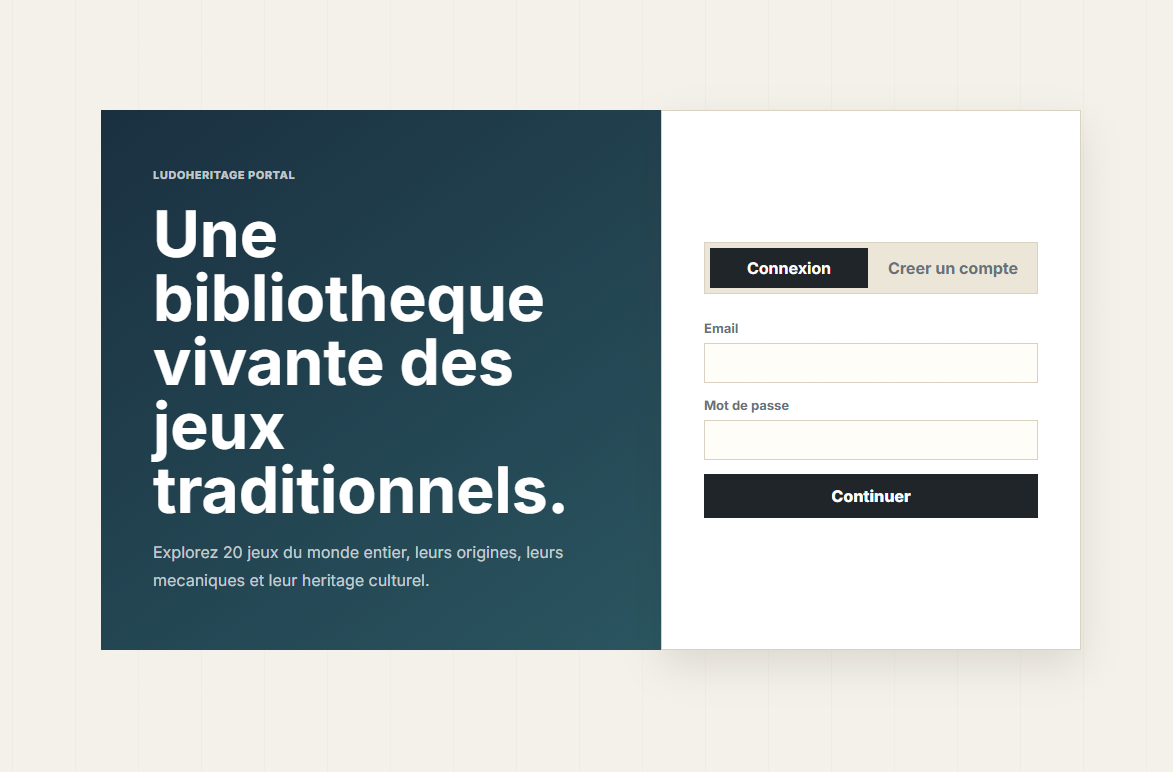
\includegraphics[angle=90, width=0.8\linewidth]{screenshots/login.png}
\caption{Pages de connexion et d'inscription -- LudoHeritage}
\end{figure}
\begin{figure}[H]
\centering
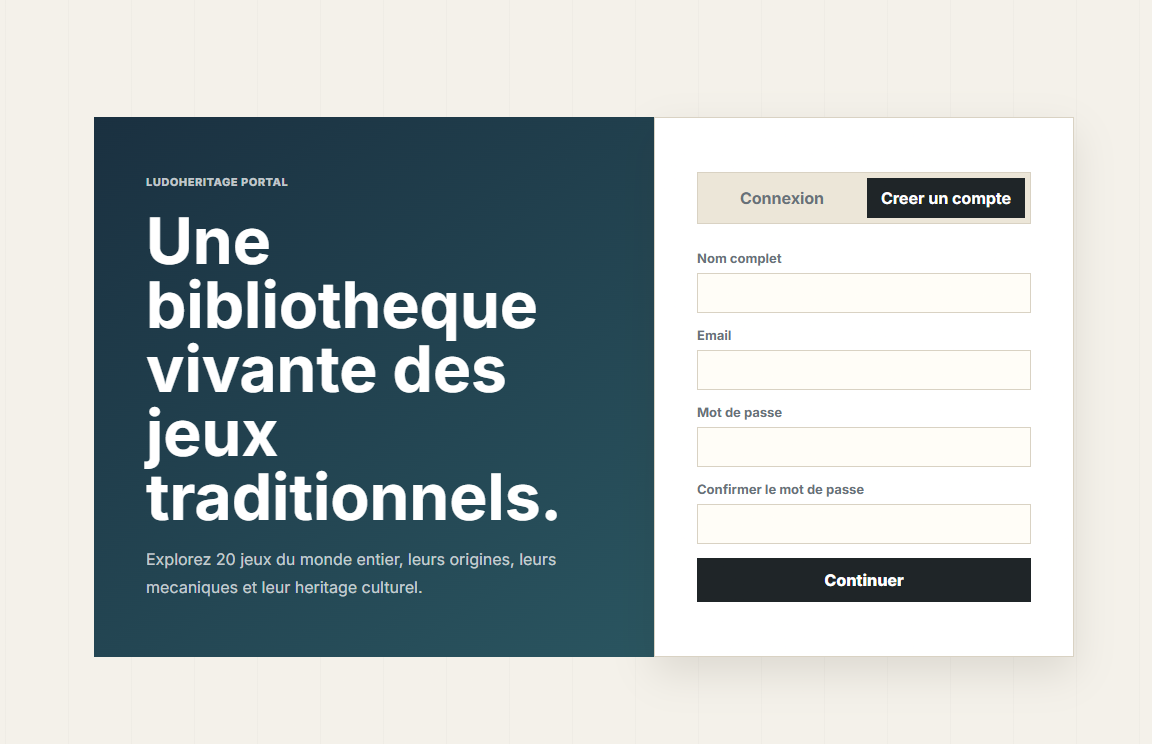
\includegraphics[angle=90, width=1\linewidth]{screenshots/signup.png}
\caption{Pages de connexion et d'inscription -- LudoHeritage}
\end{figure}
La page d'authentification adopte une mise en page en deux colonnes~: à gauche, un panneau
de présentation de la plateforme~; à droite, le formulaire de connexion ou d'inscription.
L'inscription ne requiert qu'un nom, une adresse e-mail et un mot de passe.

\begin{figure}[H]
\centering
\includegraphics[width=0.8\linewidth]{images/qst1.png}
\caption{Questionnaire de bienvenue en quatre étapes}
\end{figure}

Lors de sa première connexion, l'utilisateur répond à un questionnaire de bienvenue en
quatre questions portant sur son niveau de jeu, son type préféré, la région qui l'intéresse
et la langue de discussion souhaitée avec LudoBot. Ce profilage initial permet à l'assistant
de personnaliser ses recommandations dès le départ.

\subsection{Le catalogue des jeux}

\begin{figure}[H]
\centering
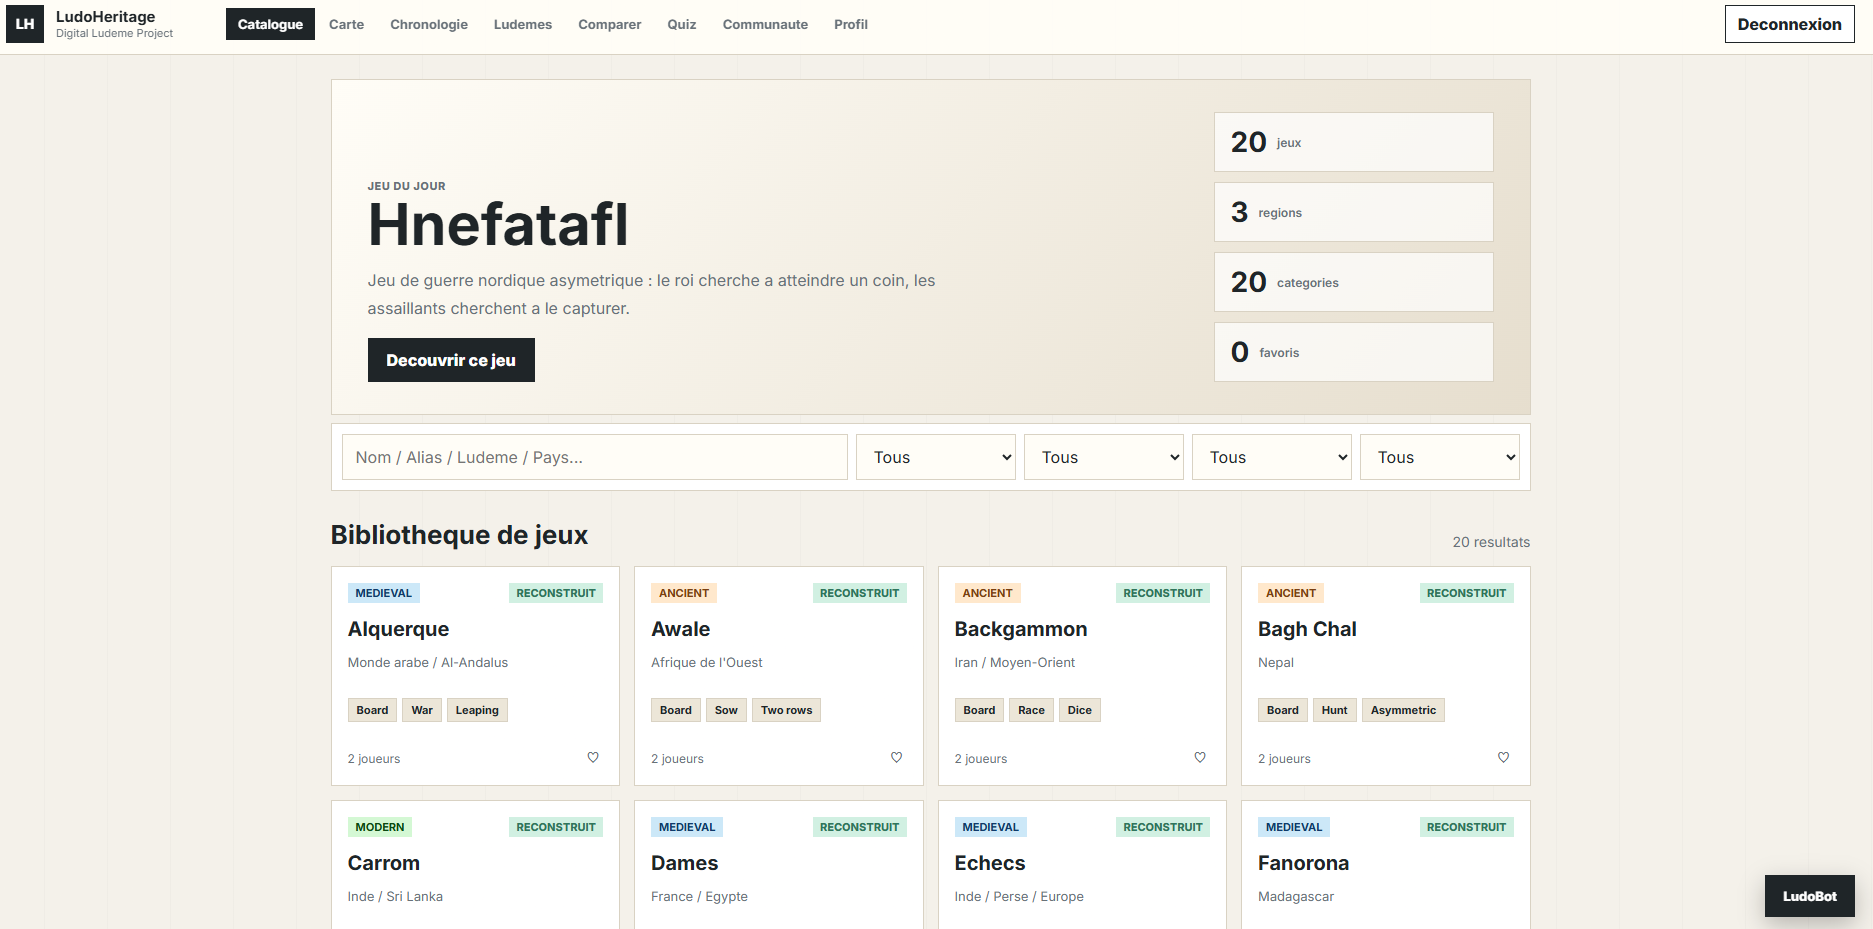
\includegraphics[angle=90,width=0.7\linewidth]{screenshots/catalogue.png}
\caption{Catalogue des jeux avec filtres actifs}
\end{figure}

Le catalogue présente les vingt jeux sous forme de cartes visuelles, accompagnées d'une
barre de filtres selon cinq critères~: région, époque, nombre de joueurs, complexité et
type de mécanique.



\subsection{La carte mondiale interactive}

\begin{figure}[H]
\centering
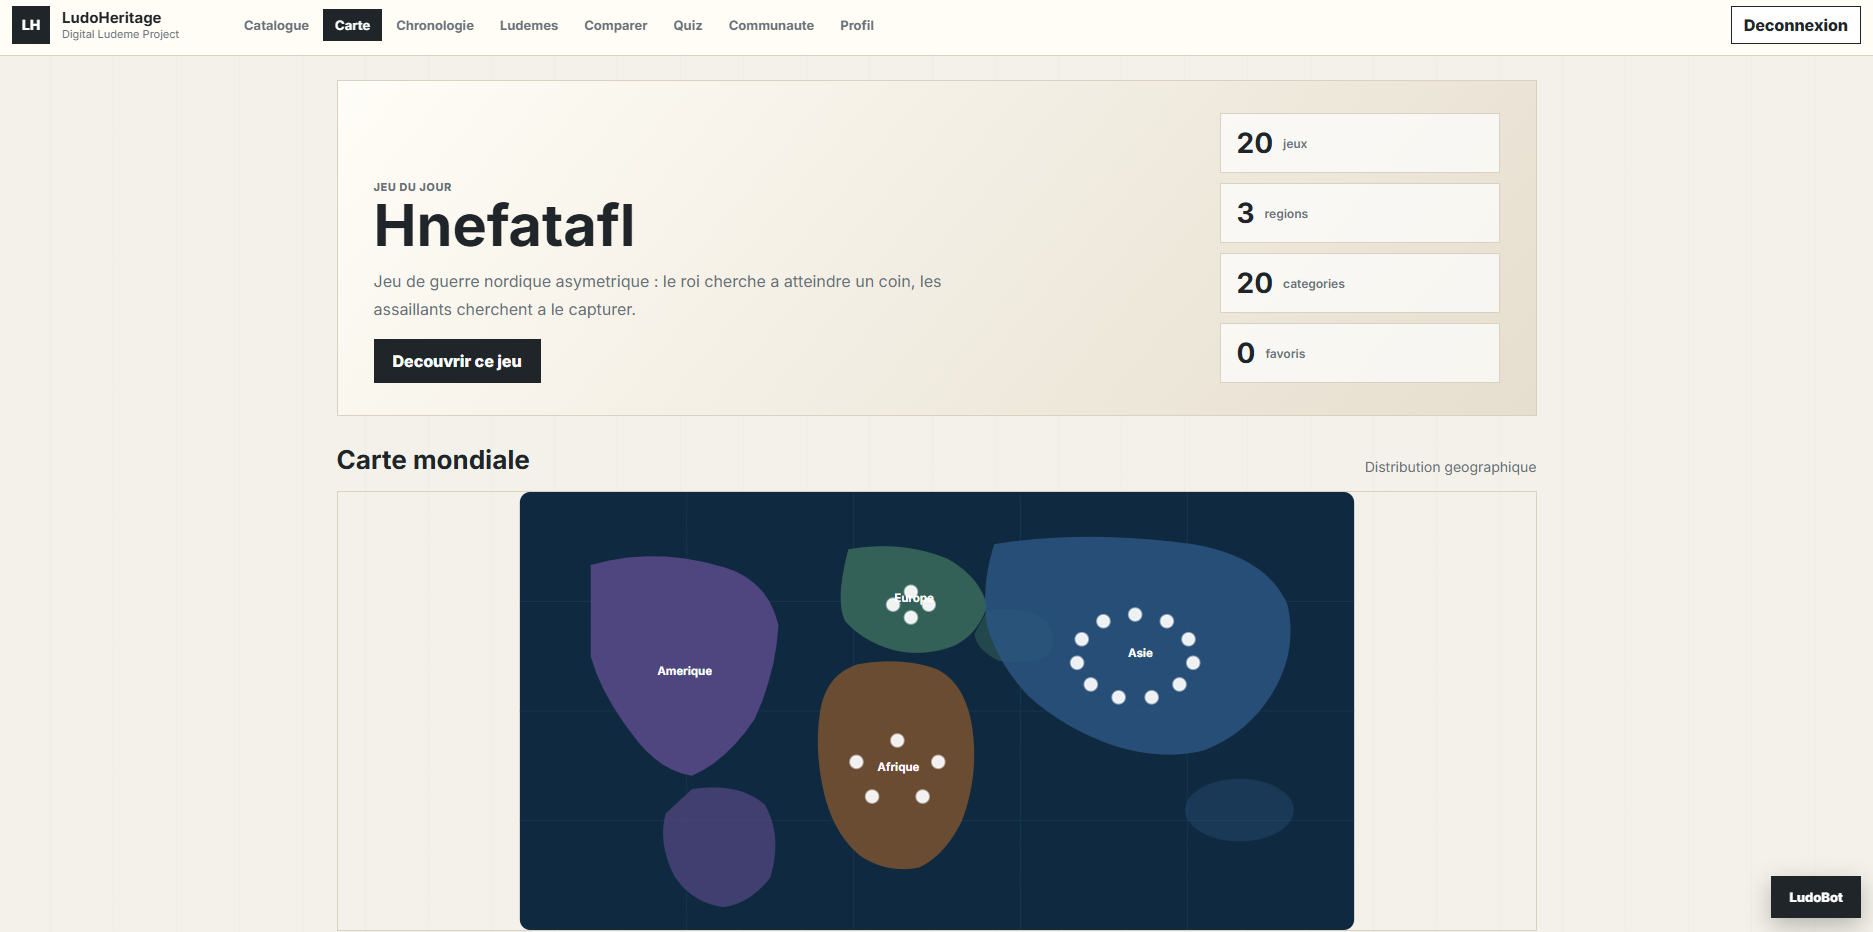
\includegraphics[angle=90,width=0.7\linewidth]{screenshots/carte.png}
\caption{Carte mondiale -- les jeux positionnés sur leurs régions d'origine}
\end{figure}

La page Carte propose une exploration géographique du catalogue. Chaque jeu est représenté
par un marqueur positionné sur sa région d'origine. Un clic sur ce marqueur affiche un
résumé du jeu et un lien vers sa fiche complète.

\subsection{La chronologie historique}

\begin{figure}[H]
\centering
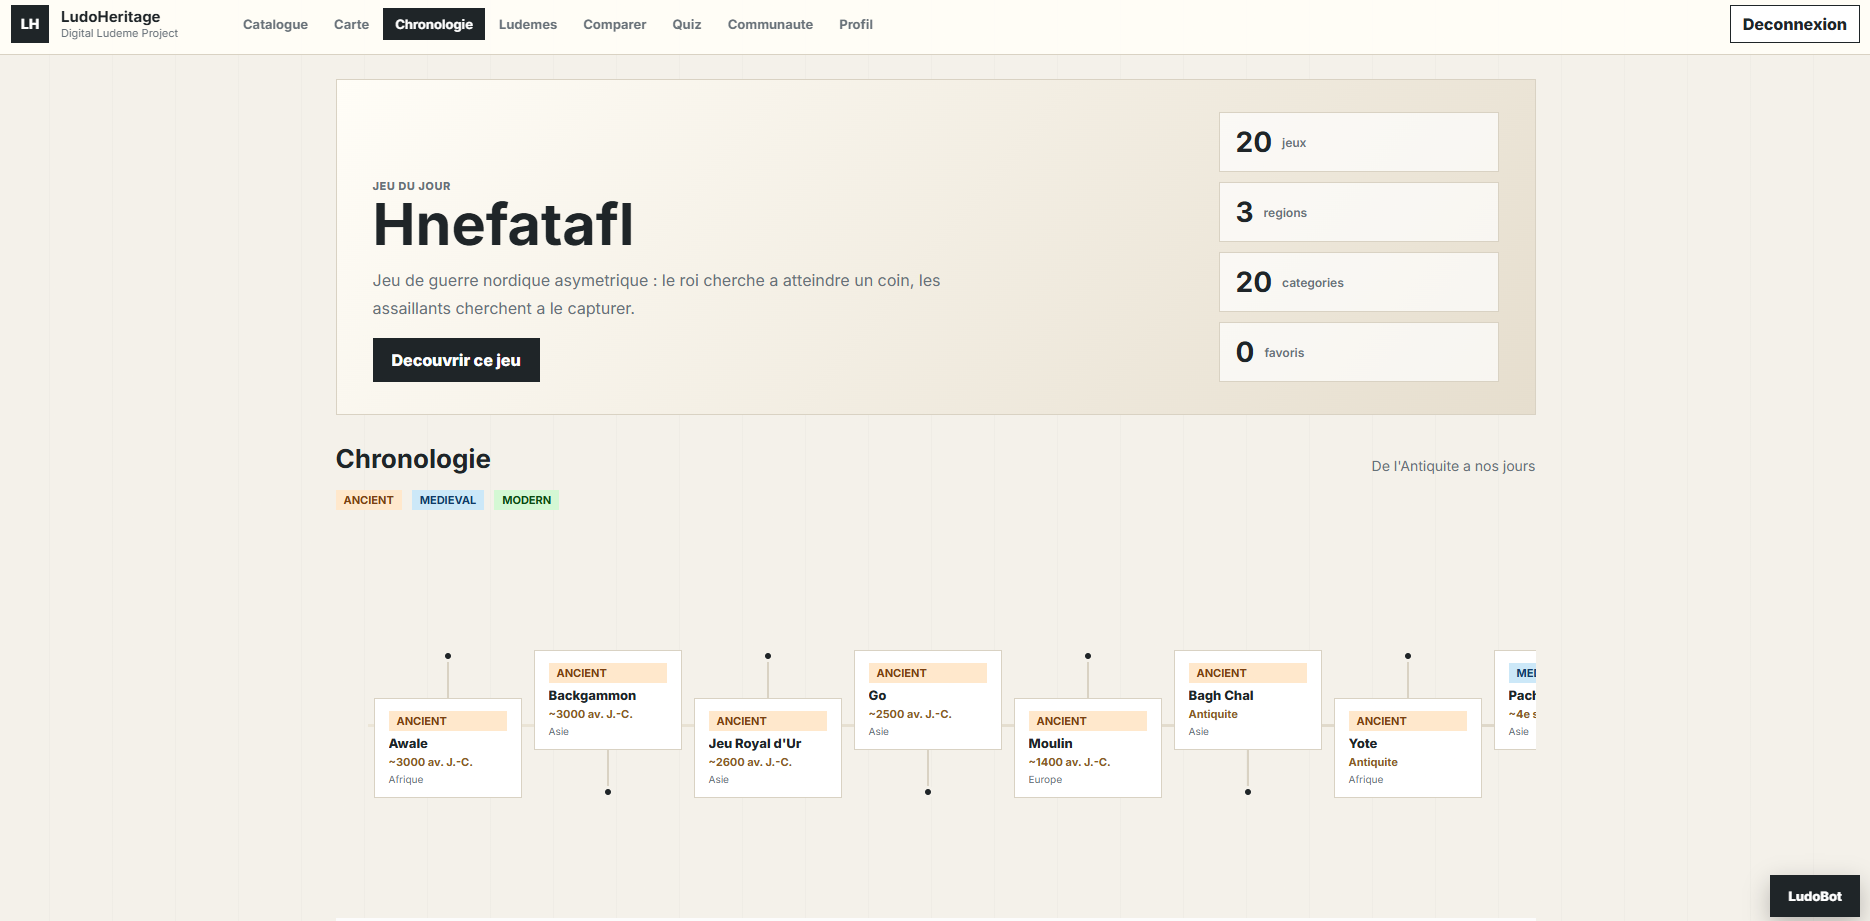
\includegraphics[angle=90,width=0.6\linewidth]{screenshots/chronologie.png}
\caption{Chronologie historique -- de l'Antiquité à l'époque moderne}
\end{figure}

La Chronologie place les vingt jeux sur une frise temporelle horizontale défilante,
du plus ancien -- le Jeu Royal d'Ur, vers 2600 avant J.-C. -- au plus récent -- le
Carrom, vers 1800. Cette mise en perspective temporelle permet de saisir l'étendue
historique du patrimoine ludique humain.

\subsection{L'outil de comparaison}

\begin{figure}[H]
\centering
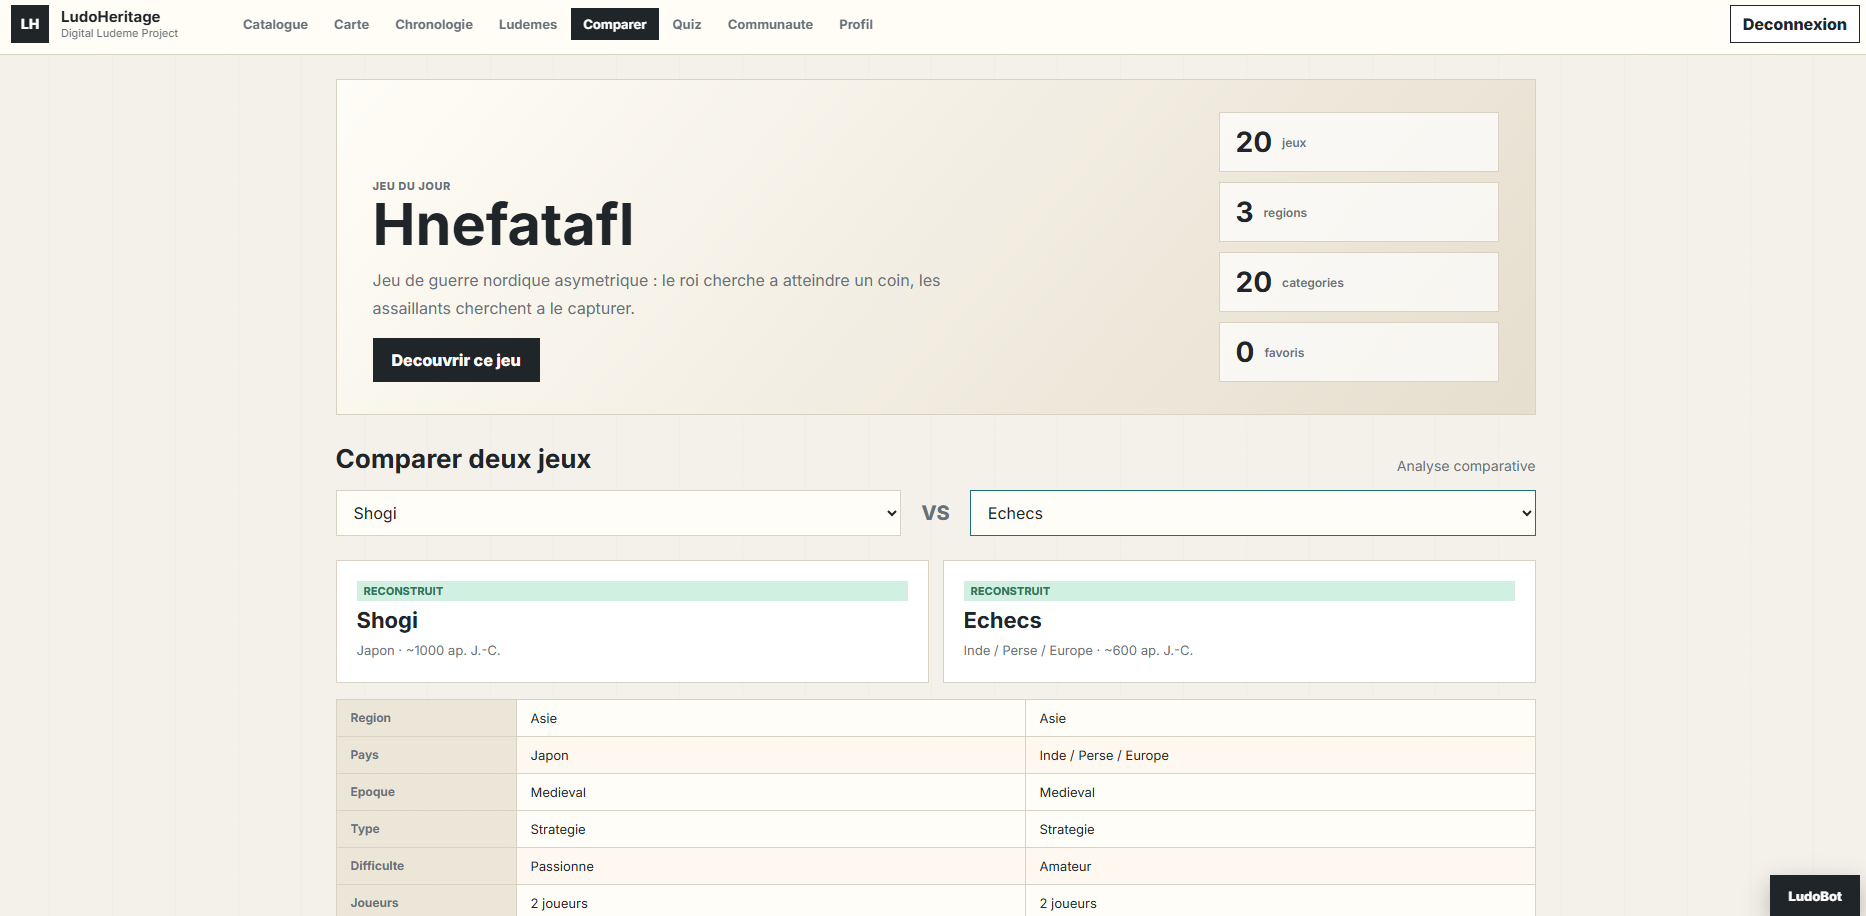
\includegraphics[angle=90 ,width=0.6\linewidth]{screenshots/comparaison.png}
\caption{Comparaison de deux jeux -- différences et points communs}
\end{figure}

L'outil de comparaison permet de placer deux jeux côte à côte pour une analyse comparative.
Les mécaniques communes apparaissent en surbrillance verte, facilitant l'identification
des similitudes culturelles entre des jeux de civilisations différentes.

\subsection{Le module Quiz}

\begin{figure}[H]
\centering
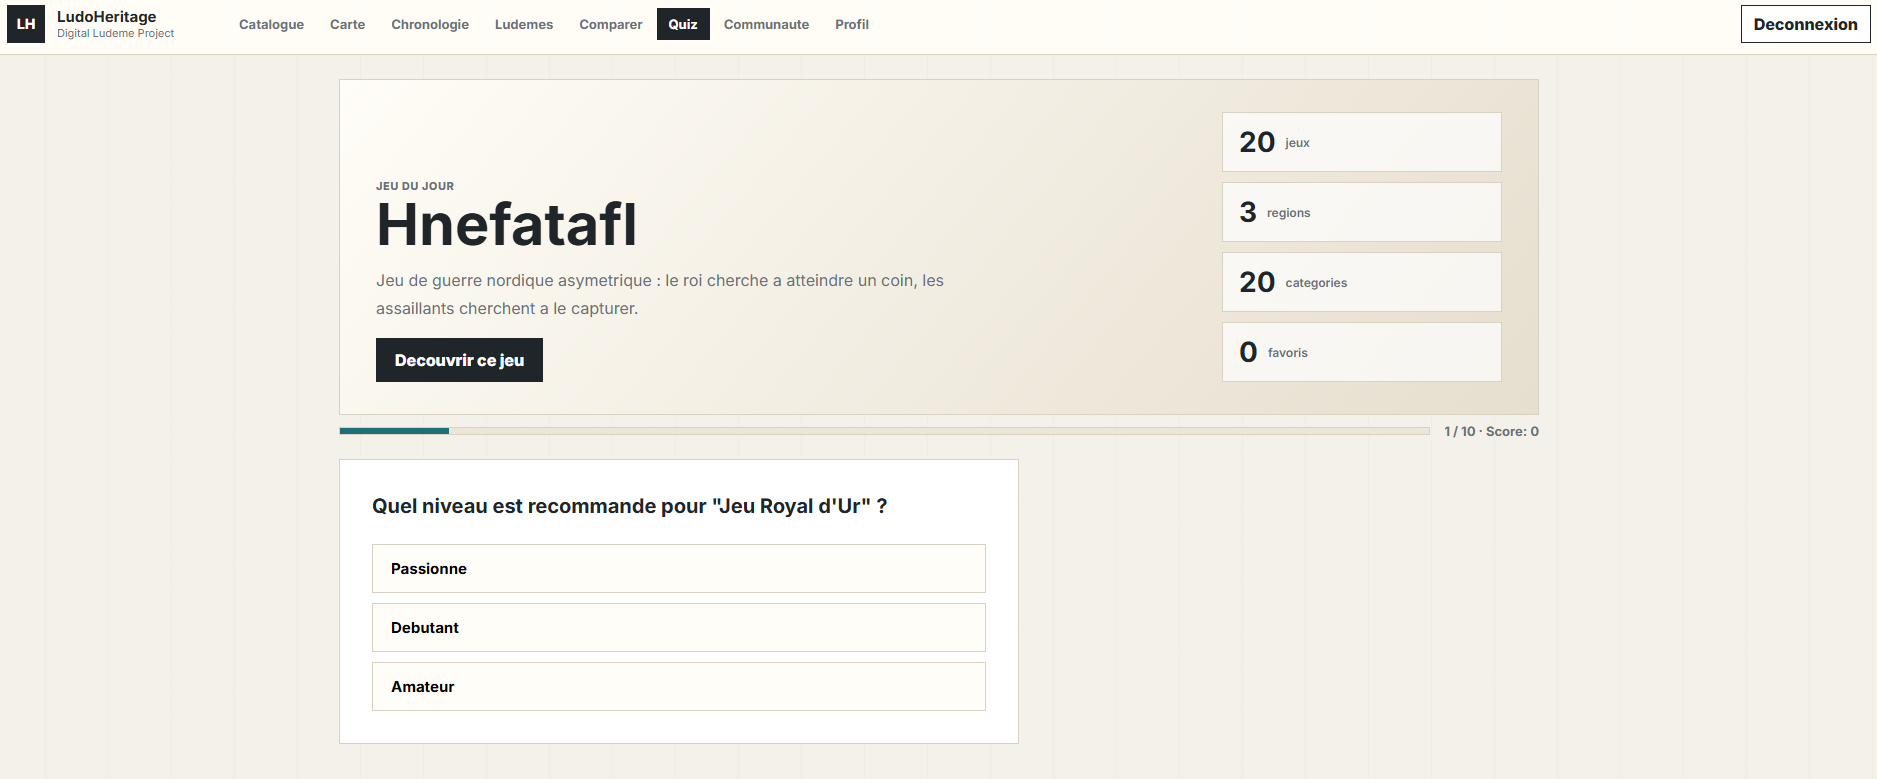
\includegraphics[angle=90,width=0.5\linewidth]{screenshots/quiz.png}
\caption{Module Quiz -- questions interactives et classement}
\end{figure}

Le module Quiz propose des sessions de dix questions à choix multiples sur les jeux du
catalogue. La correction s'affiche immédiatement après chaque réponse. À l'issue de la
session, le score est enregistré dans le classement en ligne consultable par tous les
utilisateurs.

\subsection{Le forum communautaire}

\begin{figure}[H]
\centering
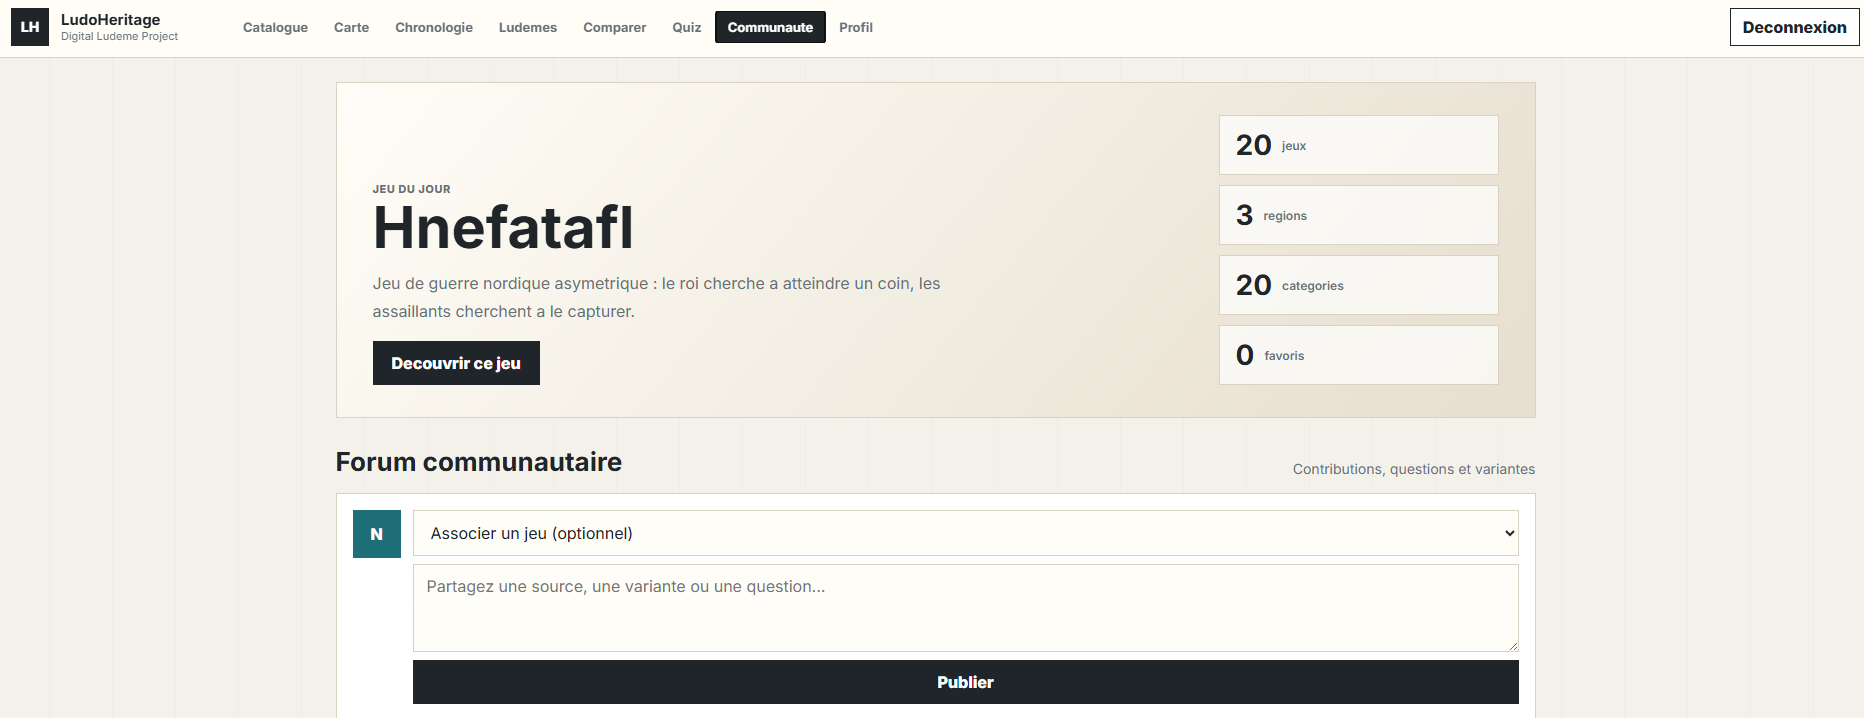
\includegraphics[angle=90, width=0.55\linewidth]{screenshots/commauntie.png}
\caption{Forum communautaire -- échanges entre passionnés}
\end{figure}

Le forum permet aux utilisateurs inscrits de partager leurs découvertes, de poser des
questions et d'échanger avec d'autres passionnés de jeux traditionnels. Chaque fil de
discussion est lié à un jeu du catalogue ou à une thématique libre.

\subsection{Le profil utilisateur}

\begin{figure}[H]
\centering
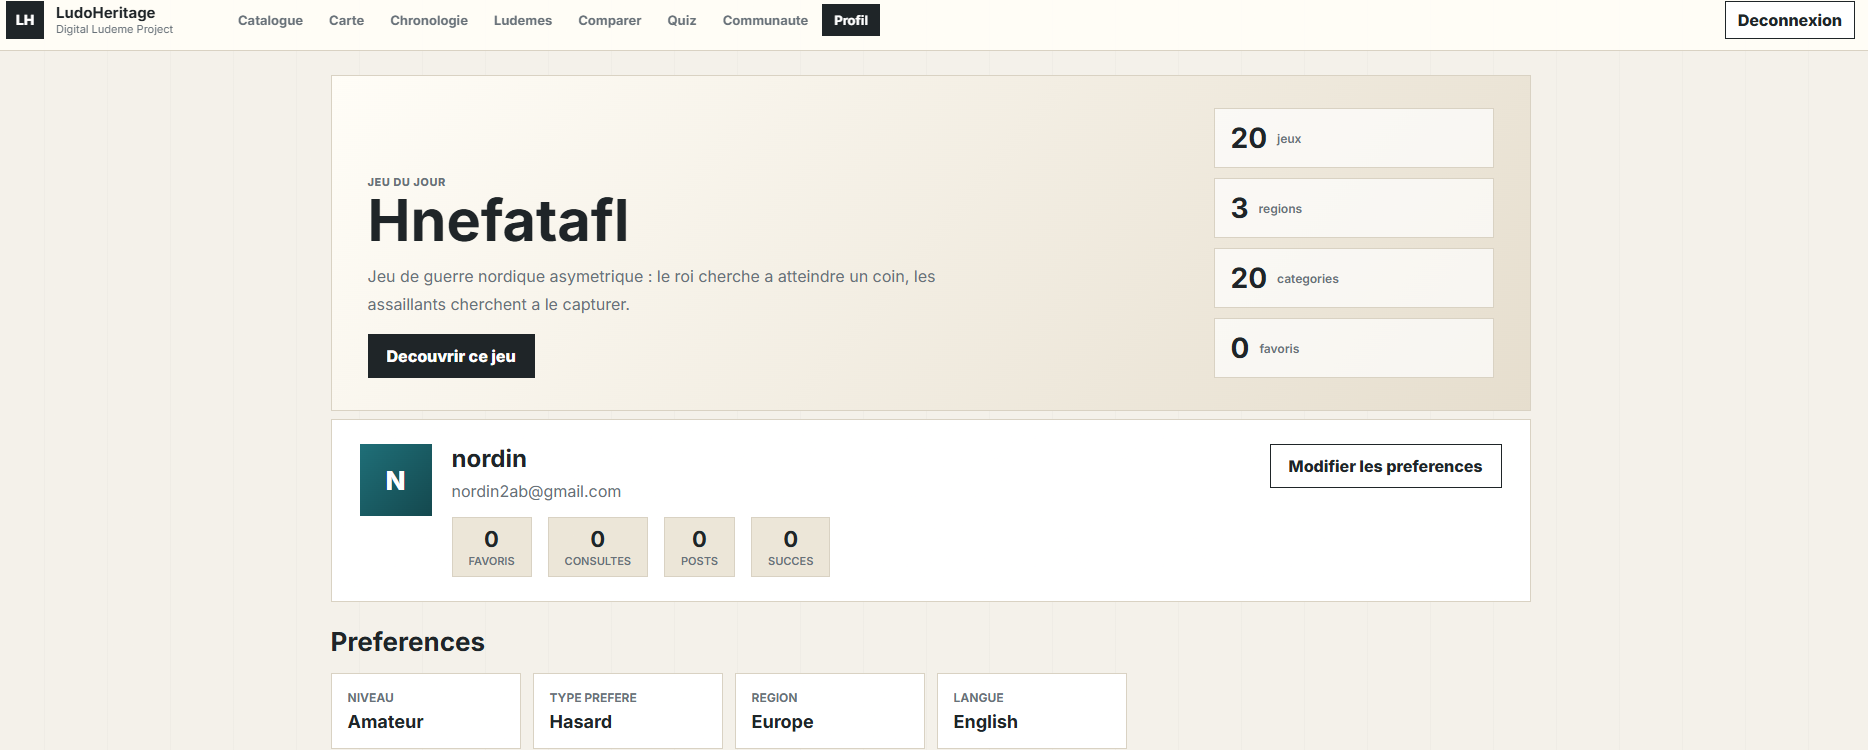
\includegraphics[angle=90, width=0.5\linewidth]{screenshots/profil.png}
\caption{Page Profil -- espace personnel avec succès et recommandations}
\end{figure}

La page Profil centralise les statistiques de l'utilisateur, ses jeux favoris, son
historique de quiz et les succès débloqués. Elle affiche également les recommandations
personnalisées générées par LudoBot sur la base du profil établi lors du questionnaire
de bienvenue.

\subsection{LudoBot, l'assistant IA}

\begin{figure}[H]
\centering
\includegraphics[width=0.9\linewidth]{images/botai.png}
\caption{LudoBot -- assistant IA intégré dans la plateforme}
\end{figure}

LudoBot est accessible depuis un bouton flottant situé en bas à droite de toutes les
pages. Il comprend les questions formulées en langage naturel, consulte le profil de
l'utilisateur et le catalogue, et propose des recommandations adaptées. En cas
d'indisponibilité du moteur IA, une réponse de secours cohérente est générée automatiquement.


\section{Conclusion}

Ce chapitre a présenté les outils techniques retenus pour la réalisation de LudoHeritage
ainsi que les principales interfaces de la plateforme. L'ensemble des fonctionnalités
décrites a fait l'objet de tests rigoureux, présentés dans le chapitre suivant.

%=============================================================================
%  CHAPITRE 4
%=============================================================================
\chapter{Tests et Validation}

\section{Introduction}

Développer une application ne suffit pas~: il faut s'assurer qu'elle fonctionne
correctement dans toutes les situations. Pour valider LudoHeritage, nous avons mis en
place une stratégie de test à trois niveaux~: des tests unitaires, des tests d'intégration
et des tests de stress. Au total, \textbf{53 tests automatisés} ont été écrits et
exécutés avec Maven, et tous passent sans aucun échec.

\section{Tests unitaires}

Les tests unitaires vérifient chaque service de manière isolée, sans base de données
ni serveur. Les dépendances externes sont remplacées par des doublures de test
(\textit{mocks}) grâce à Mockito, ce qui permet de tester la logique métier seule,
rapidement et de façon fiable.

Le service d'authentification a été testé à travers neuf cas couvrant l'inscription,
la connexion et le questionnaire de bienvenue. On vérifie notamment que l'adresse
e-mail est toujours normalisée en minuscules, que le mot de passe est systématiquement
chiffré avec BCrypt avant d'être sauvegardé, et que les erreurs comme un e-mail déjà
utilisé ou un utilisateur introuvable déclenchent bien les codes HTTP appropriés
(409 Conflict et 404 Not Found).

Le service des jeux a quant à lui été testé à travers dix-sept cas portant sur les
filtres, les tris, la recherche par mot-clé et les fonctionnalités spéciales. On
confirme par exemple que le catalogue retourne bien les vingt jeux sans filtre, que les
résultats sont triés alphabétiquement, que le jeu du jour est déterministe pour une
même date, et que la recherche par identifiant inconnu retourne une réponse vide sans
planter.

\begin{figure}[H]
\centering

\includegraphics[width=1\linewidth]{images/fig_test_counts.png}
\caption{Répartition des 53 tests par classe et par type}
\label{fig:test-counts}
\end{figure}

\section{Tests d'intégration}

Les tests d'intégration vérifient que les contrôleurs REST répondent correctement
aux requêtes HTTP, en utilisant MockMvc pour simuler de vraies requêtes sans démarrer
le serveur. Vingt-quatre tests répartis sur trois contrôleurs ont été réalisés.

Pour le contrôleur d'authentification, on s'assure que les formulaires mal remplis
sont rejetés avec un code 400, qu'un e-mail déjà existant déclenche un 409, et qu'un
mauvais mot de passe retourne un 401. Pour le contrôleur des jeux, tous les points
d'accès sont testés~: liste globale, filtres, accès par identifiant, jeu du jour et
recherche. Un identifiant inexistant retourne bien un 404. Pour le contrôleur du quiz,
on vérifie que la soumission d'un score est correctement enregistrée et que le
classement est renvoyé, même lorsqu'il est vide.

Ces tests confirment que la couche web de LudoHeritage se comporte exactement comme
attendu~: les données valides passent, les données incorrectes sont rejetées avec le
bon message d'erreur.

\begin{figure}[H]
\centering

\includegraphics[width=0.7\linewidth]{images/fig_test_donut.png}
\caption{Taux de réussite global~: 53 tests sur 53 passés}
\label{fig:test-donut}
\end{figure}

\section{Tests de stress}

Les tests de stress mesurent le comportement du catalogue de jeux lorsque de nombreux
utilisateurs accèdent au service en même temps. Trois scénarios ont été joués~: le
premier lance 50 threads qui appellent chacun la méthode \texttt{getAllGames} cent
fois de suite (5\,000 appels au total)~; le deuxième simule 50 threads effectuant des
opérations variées comme la recherche, la récupération par identifiant et le jeu du
jour (3\,000 appels)~; le troisième soumet 30 threads à des recherches et filtres
aléatoires (2\,400 appels).

Sur les \textbf{10\,400 appels concurrents} réalisés, le taux d'erreur est de
\textbf{0\,\%} dans les trois scénarios. La latence moyenne reste inférieure à
\textbf{1\,ms}, et même le 99\textsuperscript{e} percentile ne dépasse pas 11\,ms.
Ces résultats montrent que le mécanisme de catalogue en mémoire est parfaitement
adapté à une utilisation concurrente~: aucun blocage, aucune corruption de données,
des réponses rapides et stables quelle que soit la charge.

\begin{figure}[H]
\centering

\includegraphics[width=1\linewidth]{images/fig_stress_latency.png}
\caption{Latences des tests de stress~: moyenne, P95 et P99 par scénario}
\label{fig:stress-latency}
\end{figure}

\begin{figure}[H]
\centering

\includegraphics[width=1\linewidth]{images/fig_stress_throughput.png}
\caption{Volume d'appels et taux d'erreur sous charge concurrente}
\label{fig:stress-throughput}
\end{figure}

\section{Bilan global}

L'ensemble des 53 tests s'exécute en moins de six secondes au total, ce qui montre
que la suite de tests est légère et peut être relancée à tout moment sans perte de
temps. Les tests unitaires sont les plus rapides (moins de 400\,ms pour 26 tests),
tandis que les tests d'intégration prennent un peu plus de temps car ils démarrent
un contexte Spring. La figure suivante illustre les durées par classe de test.

\begin{figure}[H]
\centering

\includegraphics[width=1\linewidth]{images/fig_exec_time.png}
\caption{Durée d'exécution de chaque classe de test}
\label{fig:exec-time}
\end{figure}

\begin{figure}[H]
\centering

\includegraphics[width=1\linewidth]{images/fig_dashboard.png}
\caption{Tableau de bord global des tests et des performances}
\label{fig:dashboard}
\end{figure}

\section{Sécurité}

La sécurité de la plateforme repose sur trois mesures qui ont toutes été validées
par les tests. Les mots de passe ne sont jamais stockés en clair~: l'algorithme
BCrypt transforme chaque mot de passe en empreinte cryptographique avant toute
sauvegarde, ce qui a été vérifié par un test unitaire dédié. Toutes les données
envoyées par l'utilisateur sont validées côté serveur~: les tests d'intégration
ont confirmé que les requêtes malformées reçoivent un code 400 sans que le serveur
n'exécute aucune opération. Enfin, les erreurs sont gérées de façon centralisée~:
elles sont transformées en messages lisibles pour l'utilisateur, sans jamais
exposer les détails internes du système.

\section{Conclusion}

Ce chapitre a montré que LudoHeritage est une application correcte, robuste et
performante. Les 53 tests automatisés couvrent les comportements normaux et les
cas d'erreur, à tous les niveaux de l'application. Les résultats sous charge
confirment que la plateforme peut servir de nombreux utilisateurs simultanément
sans aucune dégradation. Le chapitre suivant explore les pistes d'amélioration
envisagées pour faire évoluer LudoHeritage au-delà de sa version actuelle.

%=============================================================================
%  CHAPITRE 5
%=============================================================================
\chapter{Perspectives et Améliorations}

\section{Introduction}

LudoHeritage est aujourd'hui une plateforme fonctionnelle et complète. Cependant, toute
application mérite d'évoluer pour mieux répondre aux attentes de ses utilisateurs et
s'adapter aux nouvelles technologies. Ce chapitre présente les pistes d'amélioration
envisagées pour les versions futures.

\section{Améliorations techniques}

Plusieurs évolutions techniques sont prioritaires. En matière d'\textbf{authentification},
la mise en place d'un système de jetons JWT avec renouvellement automatique renforcerait
la sécurité des sessions. Un \textbf{panneau d'administration} plus complet permettrait
de gérer le catalogue sans nécessiter d'intervention directe dans le code. Enfin, le
\textbf{déploiement en production} sur une infrastructure cloud rendrait la plateforme
accessible à un public mondial.

\section{Améliorations fonctionnelles}

Sur le plan fonctionnel, plusieurs axes d'enrichissement sont envisagés. L'ajout de
\textbf{jeux jouables} supplémentaires -- le Moulin et le Mancala notamment -- élargirait
l'expérience interactive. Un \textbf{contenu multilingue}, avec des traductions en anglais
et en arabe, permettrait de toucher un public plus large. Les \textbf{contributions
communautaires}, sous forme de soumissions de variantes avec un système de modération,
favoriseraient l'engagement des utilisateurs. Enfin, une \textbf{nouvelle génération de
LudoBot} disposant d'une mémoire de conversation et d'une détection automatique de la
langue améliorerait considérablement l'expérience de dialogue.

\section{Extension du catalogue}

Le catalogue de vingt jeux pourrait être progressivement étendu à cinquante, voire cent
entrées, avec une attention particulière portée aux jeux régionaux marocains et
maghrébins, encore peu représentés dans les ressources numériques francophones.

\section{Conclusion}

Les perspectives présentées dans ce chapitre témoignent du potentiel d'évolution de
la plateforme. Les priorités pour les versions futures sont le déploiement en production,
le contenu multilingue et l'extension du catalogue, qui constituent les leviers les plus
impactants pour la croissance de LudoHeritage.

%=============================================================================
%  CONCLUSION GENERALE
%=============================================================================
\newpage
\chapter*{Conclusion Générale}
\addcontentsline{toc}{chapter}{Conclusion Générale}
\thispagestyle{fancy}

Ce projet nous a permis de concevoir et de mettre en place une plateforme web de
préservation du patrimoine ludique mondial, offrant aux utilisateurs un accès interactif
et accessible aux jeux traditionnels en langue française.

Depuis l'analyse des besoins jusqu'à la réalisation et la validation, nous avons parcouru
l'ensemble du cycle de développement d'un projet logiciel. Cette expérience nous a permis
d'appliquer concrètement les connaissances acquises au cours de notre formation~: conception
UML, architecture MVC, framework Spring Boot, développement frontend avec React, intégration
d'une intelligence artificielle locale avec Ollama, et gestion de données avec MongoDB.

Au-delà des aspects techniques, ce projet nous a conduits à développer notre capacité à
travailler en équipe, à communiquer efficacement et à résoudre des problèmes complexes
en situation réelle. Les difficultés rencontrées -- qu'elles soient liées à l'intégration
des composants, à la gestion des cas d'erreur ou à la qualité de l'interface -- ont été
autant d'occasions d'apprendre et de progresser.

LudoHeritage n'est pas seulement un projet académique~: c'est une contribution, modeste
mais sincère, à la valorisation d'un patrimoine culturel trop souvent négligé dans l'espace
numérique francophone.

%=============================================================================
%  BIBLIOGRAPHIE
%=============================================================================
\newpage
\chapter*{Bibliographie}
\addcontentsline{toc}{chapter}{Bibliographie}
\thispagestyle{fancy}

\begin{enumerate}
  \item Documentation officielle Spring Boot -- \textit{https://spring.io/projects/spring-boot}
  \item Documentation officielle React -- \textit{https://react.dev/}
  \item Documentation officielle MongoDB -- \textit{https://www.mongodb.com/docs/}
  \item Documentation officielle Ollama -- \textit{https://ollama.com/}
  \item Plateforme Ludii -- Digital Ludeme Project, Université de Maastricht -- \textit{https://ludii.games/}
  \item Convention UNESCO pour la Sauvegarde du Patrimoine Culturel Immatériel (2003)
  \item Documentation officielle GitHub -- \textit{https://docs.github.com/}
  \item Site officiel Stack Overflow -- \textit{https://stackoverflow.com/}
\end{enumerate}

%=============================================================================
%  ANNEXES
%=============================================================================
\newpage
\chapter*{Annexes}
\addcontentsline{toc}{chapter}{Annexes}
\thispagestyle{fancy}

\section*{Annexe A -- Structure des dossiers du projet}

\begin{verbatim}
ludoheritage/
|-- src/main/java/org/LudoHeritage/
|   |-- auth/           Gestion des comptes
|   |-- agent/          LudoBot et diagnostic Ollama
|   |-- community/      Forum communautaire
|   |-- controller/     Catalogue des jeux
|   |-- model/          Structures de donnees
|   |-- quiz/           Module quiz et classement
|   |-- service/        Logique metier et moteur IA
|   `-- config/         Configuration et gestion des erreurs
|-- src/main/resources/
|   `-- application.properties
`-- frontend/
    |-- src/
    |   |-- App.jsx
    |   `-- styles.css
    `-- package.json
\end{verbatim}

\section*{Annexe B -- Catalogue complet des 20 jeux}

\begin{table}[H]
\centering
\renewcommand{\arraystretch}{1.4}
\begin{tabular}{|p{0.5cm}|p{4.2cm}|p{4.2cm}|p{3cm}|}
\hline
\rowcolor{mainblue!20}
\textbf{N°} & \textbf{Jeu} & \textbf{Région / Pays} & \textbf{Époque} \\
\hline
1  & Awalé          & Afrique de l'Ouest   & Ancien    \\ \hline
2  & Mancala        & Afrique de l'Est     & Ancien    \\ \hline
3  & Backgammon     & Iran / Moyen-Orient  & Ancien    \\ \hline
4  & Go             & Chine                & Ancien    \\ \hline
5  & Échecs         & Inde / Perse         & Médiéval  \\ \hline
6  & Dames          & France / Égypte      & Médiéval  \\ \hline
7  & Shogi          & Japon                & Médiéval  \\ \hline
8  & Tablut         & Scandinavie          & Médiéval  \\ \hline
9  & Jeu Royal d'Ur & Mésopotamie          & Ancien    \\ \hline
10 & Xiangqi        & Chine                & Médiéval  \\ \hline
11 & Carrom         & Inde / Sri Lanka     & Moderne   \\ \hline
12 & Fanorona       & Madagascar           & Médiéval  \\ \hline
13 & Surakarta      & Indonésie            & Moderne   \\ \hline
14 & Moulin         & Méditerranée         & Ancien    \\ \hline
15 & Alquerque      & Monde arabe          & Médiéval  \\ \hline
16 & Toguz Korgool  & Kirghizstan          & Ancien    \\ \hline
17 & Bagh Chal      & Népal                & Ancien    \\ \hline
18 & Yoté           & Afrique de l'Ouest   & Ancien    \\ \hline
19 & Pachisi        & Inde                 & Médiéval  \\ \hline
20 & Hnefatafl      & Scandinavie          & Ancien    \\ \hline
\end{tabular}
\caption*{Catalogue complet des 20 jeux de LudoHeritage}
\end{table}

\end{document}